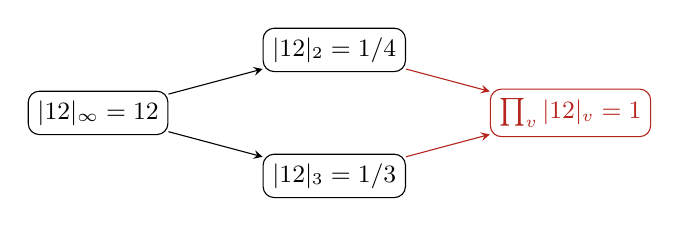
\begin{tikzpicture}[>=stealth,font=\small]
\node[draw,rounded corners] (a) at (0,0) {$|12|_\infty=12$};
\node[draw,rounded corners] (b) at (3.0,.8) {$|12|_2=1/4$};
\node[draw,rounded corners] (c) at (3.0,-.8) {$|12|_3=1/3$};
\node[draw,rounded corners,BrickRed] (d) at (6,0) {$\prod_v|12|_v=1$};
\draw[->] (a)--(b); \draw[->] (a)--(c); \draw[->,BrickRed] (b)--(d);\draw[->,BrickRed] (c)--(d);
\end{tikzpicture}
